\documentclass[
    corpo=11.5pt,
    oneside,
    evenboxes,
    tipotesi=triennale,
    stile=classica,
    oldstyle,
    autoretitolo,
    greek,
]{toptesi}
\usepackage[utf8]{inputenc}
\usepackage[T1]{fontenc}
\usepackage{lmodern}
\usepackage{hyperref}
\usepackage{setspace}
\usepackage{verbatim}
\usepackage{pgfplots}
\usepackage{graphicx}
\usepackage{subfig}
\onehalfspacing

\hypersetup{
    pdfpagemode={UseOutlines},
    bookmarksopen,
    pdfstartview={FitH},
    colorlinks,
    linkcolor={blue},
    citecolor={blue},
    urlcolor={blue}
  }
\usepackage{lipsum}

\newtheorem{osservazione}{Osservazione}

\begin{document}\errorcontextlines=9

\begin{ThesisTitlePage}
    \ateneo{Universit\`a degli Studi di Torino}
    \StrutturaDi{Dipartimento di Management}
    \struttura[]{}
    \NomeElaborato{Tesi di laurea triennale}
    \titolo{Lo stato di salute del Calcio}
    \sottotitolo{Fair Play Fiananziario e Superlega}     
    \corsodistudi{Management dell'Informazione e della Comunicazione Aziendale}
    \candidato{Riccardo \textsc{Borgo}}
    \relatore{prof.ssa ~Simona \textsc{Alfiero}}
    \sedutadilaurea{\textsc{Anno~accademico} 2021-2022}
    \logosede{img/Unito-logo, img/logo_saa.jpeg}
\end{ThesisTitlePage}

\tablespagetrue\figurespagetrue
\indici

\mainmatter
\begin{interlinea}{1.5}
    
\chapter{Introduzione generale}
Durante lo sviluppo di questa trattazione si andrà ad analizzare l'attuale "stato di salute"
del calcio europeo, di come il \emph{Financial Fair Play} abbia provato da una parte ad aiutare le società a rimanere in regola con i conti e 
dall'altra a dettare delle regole atte ad evitare comportamenti illegali da parte sopratutto dei presidenti.\\
Infine si tratterà il caso della \emph{Superlega}, per cercare di capire se questa nuova idea sia effettivamente coerente con l'epoca in cui stiamo vivendo.\\
Sopratutto a partire dall'inizio della pandemia da COVID-19 nei primi mesi del 2020 il mondo del calcio si è visto ridurre sensibilmente i ricavi, non riuscendo 
ancora oggi ad operare al 100\%. Grazie, forse, a questa situazione di difficoltà è stato evidenziato come la situazione odierna non fosse più sostenibile: 
club con milioni di euro di debiti, richieste di ingaggio "faraoniche" da parte dei calciatori, con il risultato che molte societ\`a non sono state pi\`u in grado di far fronte 
a tutto questo e costrette a dichiarare falimento.\\
Il primo capitolo mira ad analizzare la situazione economica, finanziaria e patrimoniale, antecedente all'anno 2020 di alcune delle più 
importanti e storiche societ\`a di tutto il panorama europeo: Juventus per quanto riguarda l'Italia, Paris Saint Germain per quanto riguarda la 
Francia, Bayern Monaco per la Germania, Manchester City per l'Inghiterra e il Barcellona per la Spagna. I punti principali dell'analisi riguarderanno: 
Analisi dei ricavi, Analisi della liquidit\'a, Analisi della solidit\'a, Analisi della redditivit\'a e Trend azionario (se presente) in modo da 
poter fare una verifica a 360° di tutti i vari settori economici. La scelta \'e virata su queste societ\'a perch\'e per un motivo o per un altro sono state 
al centro di problematiche o scandali legate alla cattiva gestione del patrimonio oppure "accusate" di non essere state prese particolarmente prese di mira dalle misure e le leggi 
emanate nell'ultimo decennio dalla UEFA \footnote{ Union of European Football Associations}, come per esempio il \emph{Financial Fair Play}.\\
Il secondo capitolo si occuper\'a invece della presentazione e dell'analisi in modo dettagliato del \emph{Financial Fair Play} o 
\emph{FFP}, dalla sua nascita, alle varie parti presenti all'interno del documento e mostrando infine come, non sempre, tutte le societ\'a siano state trattate allo stesso modo.\\
Il terzo capitolo invece analizza invece l'impatto mediatico, non prima di aver presentato tutti i dati tecnici, di una delle ultime novità 
del mondo del calcio: la \emph{Superlega}: il nuovo modello che punta a rivoluzionare il mondo del calcio, per cercare di uscire da questa spirale di debiti
e fallimenti per cercare quindi di creare un nuovo inizio. Verr\'a mostrato in seguito se il progetto ha effettivamente preso piede all'interno del mondo del calcio 
e se è riuscito a smuovere qualcosa, portando agli occhi di tutti l'insostenibilità del modello attuale.\\
In chiusura si cercherà di determinare se i rimedi proposti dalle autorità del mondo del calcio siano stati sufficienti ad eliminare tutte le criticità presenti e 
sopratutto evidenziare l'impatto economico di questi rimedi.\\
Riuscir\'a la Superlega ad acquistare credibilità e ad affermarsi come nuovo modello, capace di risollevare il calcio?

\part{Parte Prima}
\chapter{Situazione economica Europea pre-pandemia da COVID19}
\section{Analisi generale delle diverse realt\'a Europee}
Prima di andare ad analizzare nello specifico i vari club europei \'e necessario iniziare con una prima 
parte atta a presentare come ogni paese gestisce i ricavi derivanti da questa attivit\'a. Verrà mostrato come Paesi geograficamente
molto vicini tra loro, non abbiano molti aspetti in comune da questo punto di vista, andando quindi a rendere in qualche modo 
"unico" ogni campionato con la relativa Federazione. Le Federazioni (uniche per ogni Stato) hanno tendenzialmente il compito
comune di promuovere lo sport ed eliminare ogni tipo di discriminazione; la FIGC per esempio ha come scopo e mission: 
\emph{Promuovere e disciplinare l’attività del giuoco del calcio e degli aspetti ad esso connessi, conciliando la 
dimensione professionistica con quella dilettantistica attraverso una struttura centrale e di promuovere l’esclusione dal 
giuoco del calcio di ogni forma di discriminazione sociale, razzismo, xenofobia e violenza} \footnote{https://www.figc.it/it/federazione/mission-e-governance/identita-e-missione/}. Oltre a questo compito 
pi\'u improntato sul sociale, le Federazioni hanno l'obbligo di controllare dal punto di vista finanziario le società calcistiche
dello Stato, applicando sanzioni in caso di irregolarit\'a.\\
A "capo" delle varie Federazioni troviamo la FIFA \footnote{Fédération Internationale de Football Association} che sostanzialmente 
controlla a sua volta i vari club e pu\'o applicare anch'essa sanzioni di tipo monetario o addirittura vietare partecipazioni a 
competizioni internazionali.

\subsection{Italia}
L'Italia è sempre stato un punto di riferimento fisso ed indelebile per quanto riguarda il calcio, sopratutto fino ai primi anni 2000.
Tutta l'Europa cercava di prendere esempio dal nostro Paese, sopratutto per quanto riguarda le filosofie degli allenatori, forse pi\'u
avanti come mentalità rispetto alla maggior parte dei concorrenti nel resto d'Europa. Anche i calciatori erano affascinati dal fatto di poter 
venire a giocare in Italia, perché consci di non poter far altro che trarre profitto da quella esperienza. Durante gli ultimi anni del
secolo scorso abbiamo avuto la possibilit\'a di poter veder calcare i nostri rettangoli verdi giocatori come: Gabriel Batistuta, Sinisa Mihajlovic e
Ronaldo. Anche guardando "in casa nostra", per\'o, non eravamo da meno: Alessandro Nesta, Alessandro Del Piero, Fabio Cannavaro e cos\'i via.
Dal punto di vista economico non \'e possibile rintracciare un singolo momento della storia (da trent'anni a questa parte) dove 
non si registrasse un singolo fallimento di una societ\'a. Come per le societ\'a di produzione, una squadra di calcio fallisce quando non
\'e pi\'u in grado di far fronte ai propri debiti. Solamente a partire dalla stagione 2013/2014 sono 38 i club falliti e 71 invece i club penalizzati \footnote{https://www.calcioefinanza.it/2018/07/18/fallimenti-squadre-calcio-italia/}. 
Se, invece, estendiamo il fronte temporale a partire dal 1986, come possiamo notare dalla figura \ref{fig: grafico_fallimenti} \footnote{https://www.truenumbers.it/fallimenti-calcio-italiano/}
i fallimenti delle società italiane in Lega Pro, Serie B e Serie A salgono a 175, il peggior valore tra i 5 maggiori campionati europei. 
Sono solamente 2 gli anni dove non troviamo squadre fallite (1992 e 1999), mentre il peggior valore lo troviamo nell'anno 2010 con ben 21 club andati in bancarotta
in un solo anno. Tramite la legenda \'e possibile inoltre visualizzare immediatamente come il campionato con il maggior numero di fallimenti sia
la Lega Pro con ben 165 società andate distrutte in trent'anni, questo ovviamente perch\'e i club delle leghe minori, in caso di debiti,
non hanno a disposizione magnati alle loro spalle; spesso i proprietari sono imprenditori locali che come secondo impegno gestiscono una
squadra di calcio, andando quindi in difficolt\'a quando sorgono troppe passivit\'a.

\begin{figure}
    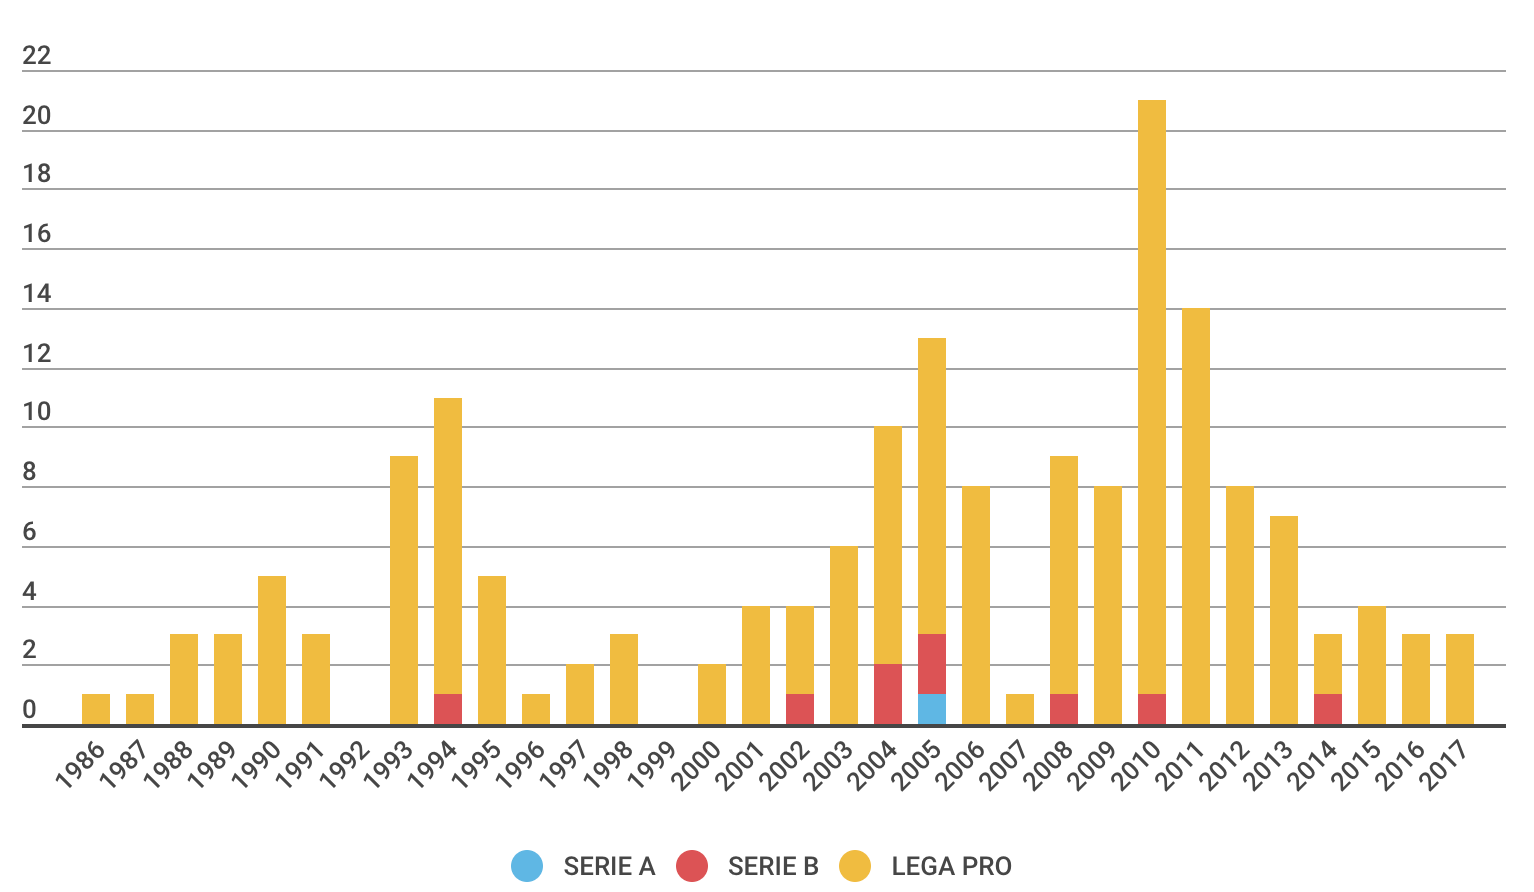
\includegraphics[scale=0.6]{img/grafico_fallimenti.png}
    \caption{Fallimenti club italiani dal 1986}
    \label{fig: grafico_fallimenti}
\end{figure}

Il motivo di tutto questo \'e possibile riassumerlo in una parola sola: \emph{malagestione}:
\'e innegabile che tutti i club abbiano delle colpe: cattivi investimenti, inequit\'a negli stipendi 
e sopratutto interessi esterni da parte dei presidenti che vedono i club come un modo per arricchirsi senza per\'o 
pensare alle conseguenze delle proprie azioni.\\
Nella figura \ref{fig: aumento_dirigenti} \footnote{https://www.truenumbers.it/squadre-calcio-italia-arbitri/} è possibile invece 
osservare come, a partire dal 2009, il numero dei dirigenti sia aumentato esponenzialmente 
rispetto a quello delle squadre affiliate alla FIGC. Questo comporta ovviamente un aumento delle spese necessarie alla remunerazione
di queste figure, andando quindi a mettere ancora più pressione alle casse dei club con minori disponibilit\'a economiche. 
In termini numerici vi \'e stato un calo generale delle societ\'a affiliate del 2,1\%: le dilettantistiche sono passate da 17157 
nel 2009 a 13593 nel 2019; le professionistiche rimangono invece pressoch\'e invariate, causa forse la maggiore disponibilit\'a 
economica che rende più facile il mantenimento di un certo numero di squadre giovanili anche in caso di risultati non remunerativi. 

\begin{figure}
    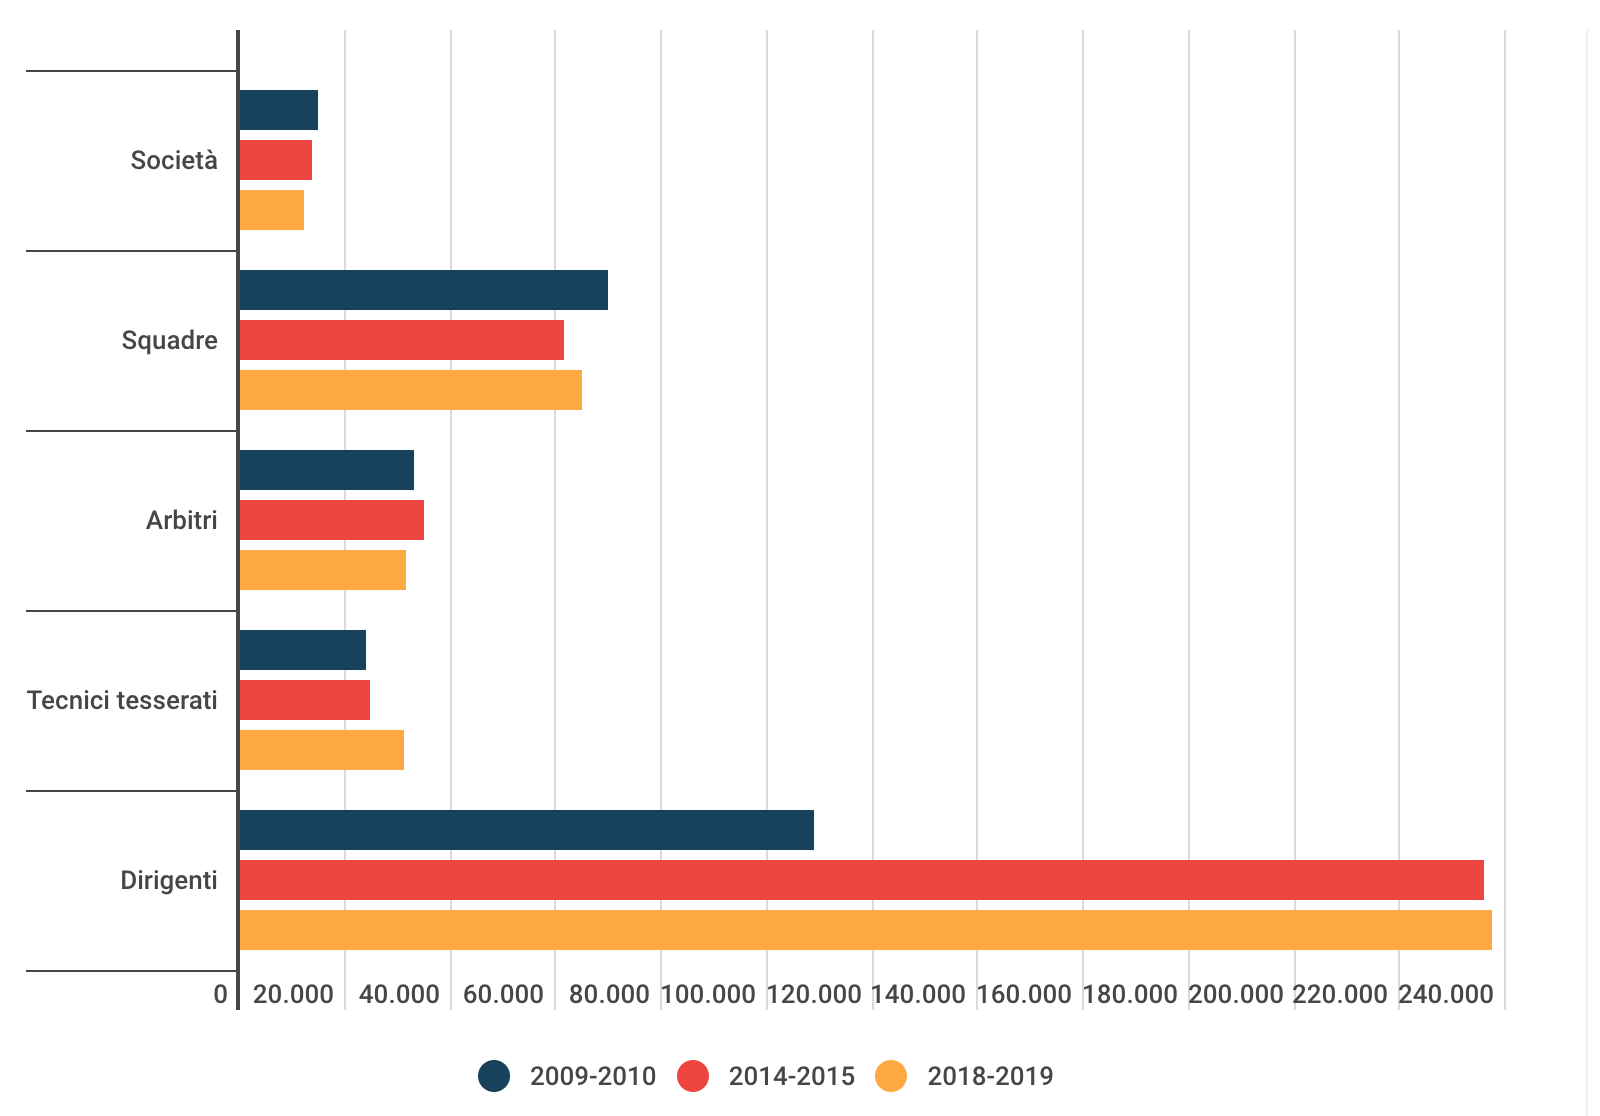
\includegraphics[scale = 0.5]{img/aumento_dirigenti.png}
    \caption{Aumento del numero di dirigenti in relazione all'aumento di club affiliati alla FIGC, a partire dalla stagione 2009-2010}
    \label{fig: aumento_dirigenti}
\end{figure}
\newpage
La tabella \ref{tabella_perdite} \footnote{https://www.calcioefinanza.it/2020/03/26/rosso-bilancio-debiti-serie-a-2018-2019/}
mostra in termini numerici i risultati di vent'anni della cosiddetta malagestione, creando, solo nella stagione 
2018/2019 300 milioni di debito e solo 8 club su 20 registranti un utile, mentre i restanti superano anche i 100 mln di euro i una singola stagione.
\begin{table}
\centering{
    \begin{tabular}{|c|c|}
        \hline
        \textbf{Club} & \textbf{Utile/Perdita (mln€)} \\
        \hline
            Napoli & +29,2 \\
            \hline
            Atalanta & +24 \\
            \hline
            Sampdoria & +12,1 \\
            \hline
            Sassuolo & +8,1 \\
            \hline
            Udinese & +1,2 \\
            \hline
            Empoli & 0,4 \\
            \hline
            Chievo & +0,01 \\
            \hline
            Spal & -0,3 \\
            \hline
            Genoa & -4 \\
            \hline
            Frosinone & -9,4 \\
            \hline
            Parma & -9,4 \\
            \hline
            Cagliari & -9,5 \\
            \hline
            Torino & -12,4 \\
            \hline
            Lazio & 13,2 \\
            \hline
            Fiorentina & -15,8 \\
            \hline
            Bologna & -21,7 \\
            \hline
            Roma & -25,1 \\
            \hline
            Juventus & -39,9 \\
            \hline
            Inter & -48,4 \\
            \hline
            Milan & -146 \\
            \hline
    \end{tabular}}
    \caption{Tabella Utile/Perdita Club Serie A stagione 2018/2019}
    \label{tabella_perdite}
\end{table}

\subsection{Francia}
Per quanto riguarda invece la Francia, l'organizzazione che si occupa del monitoraggio e la supervisione dei conti 
delle società calcistiche di associazioni di calcio in Francia è la DNCG \footnote{Direction Nationale du Contrôle de Gestion}. Essa 
pubblica ogni stagione un report riassuntivo per quanto riguarda la Ligue 1 e la Ligue 2 (i primi due campionati francesi) ed una
relazione relativa ad ogni singolo club dei due campionati. Tutti i dati di seguito riportati sono stati reperiti dai singoli
report annuali pubblicati \footnote{https://www.lfp.fr/dncg/rapports} \\
I risultati della stagione appena conclusa vengono riassunti con la figura \ref{ris_generali_2019}:
\begin{figure}
    \centering
    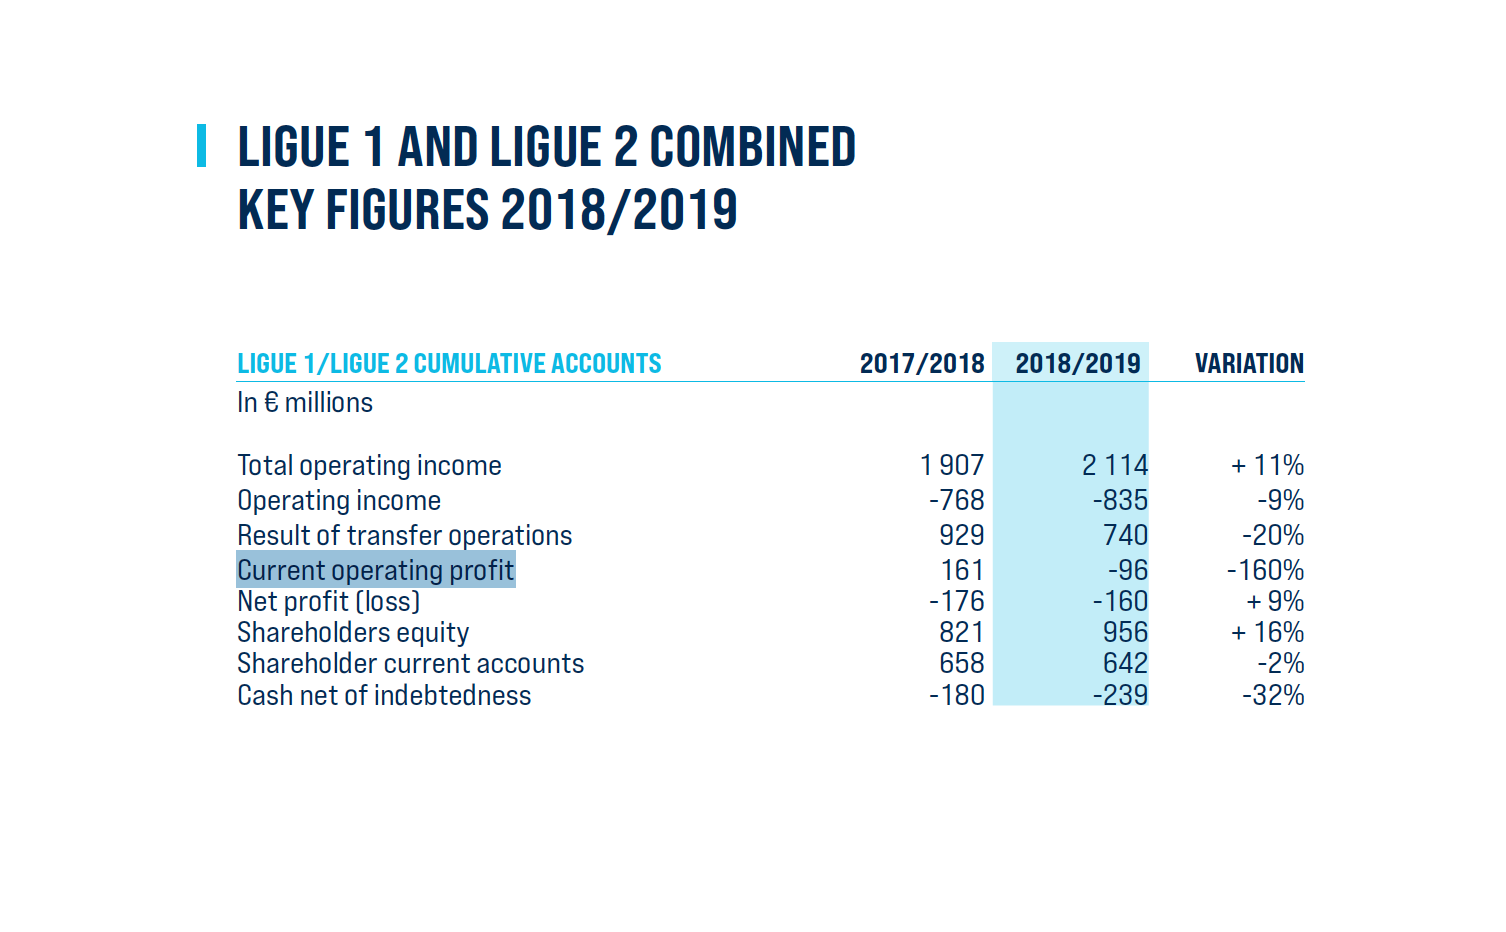
\includegraphics[scale=.5]{img/ris_generali_2019}
    \caption{Risultati generali combinati 2018/2019}
    \label{ris_generali_2019}
\end{figure}
Al termine della stagione 2018/2019 il risultato netto "consolidato" ammontava a -160 mln€, in miglioramento per\'o del 9\% rispetto 
all'anno prima (-176). Questo risultato, come indicato prima, \'e il risultato della sottrazione tra ricevi e costi d'esercizio
dei due campionati; andando ad analizzare 
nello specifico i due risultati \'e possibile notare come la Ligue 1 abbia osservato un incremento del 20\% del risultato netto
consolidato rispetto alla stagione precedente ma la Ligue 2 ha dovuto affrontare un calo del 90\% del Net Profit, andando quindi completamente
ad annullare il risultato positivo del campionato superiore. Questo risultato molto negativo \'e spiegabile tramite la comparazione 
dei grafici che mostrano la composizione del Net Income nella stagione 18/19 e precedente mostrato nella figura \ref{comp_income}.
\begin{figure}
    \centering
    \subfloat[][\emph{Composizione Net Income stagione 2017/2018}]
    {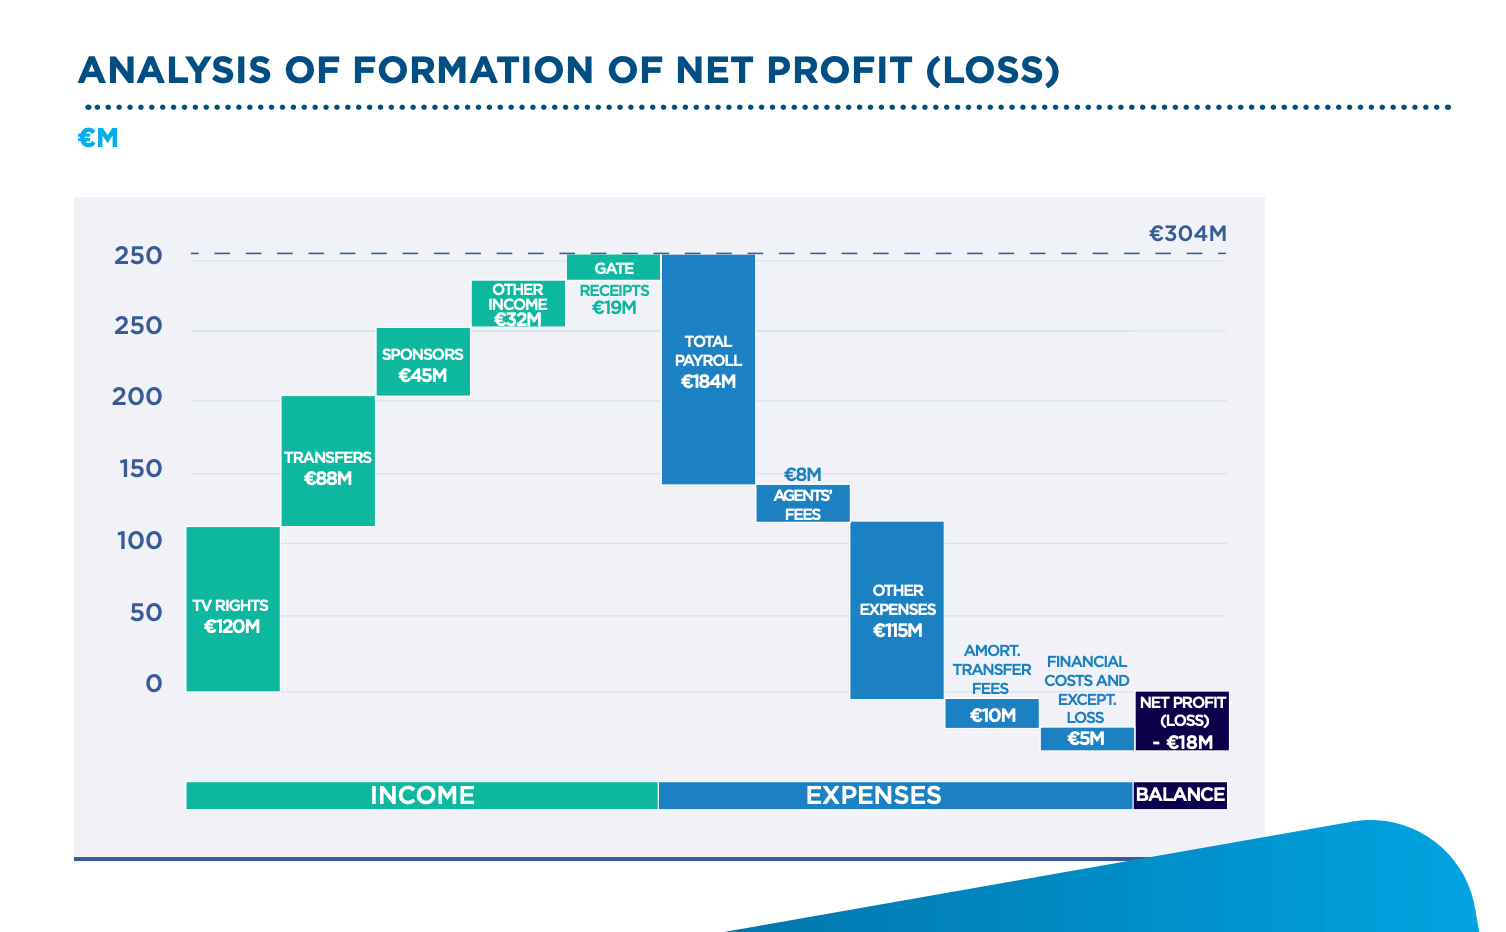
\includegraphics[width=.45\textwidth]{img/net_income_2018.png}} \quad
    \subfloat[][\emph{Composizione Net Income stagione 2017/2018}]
    {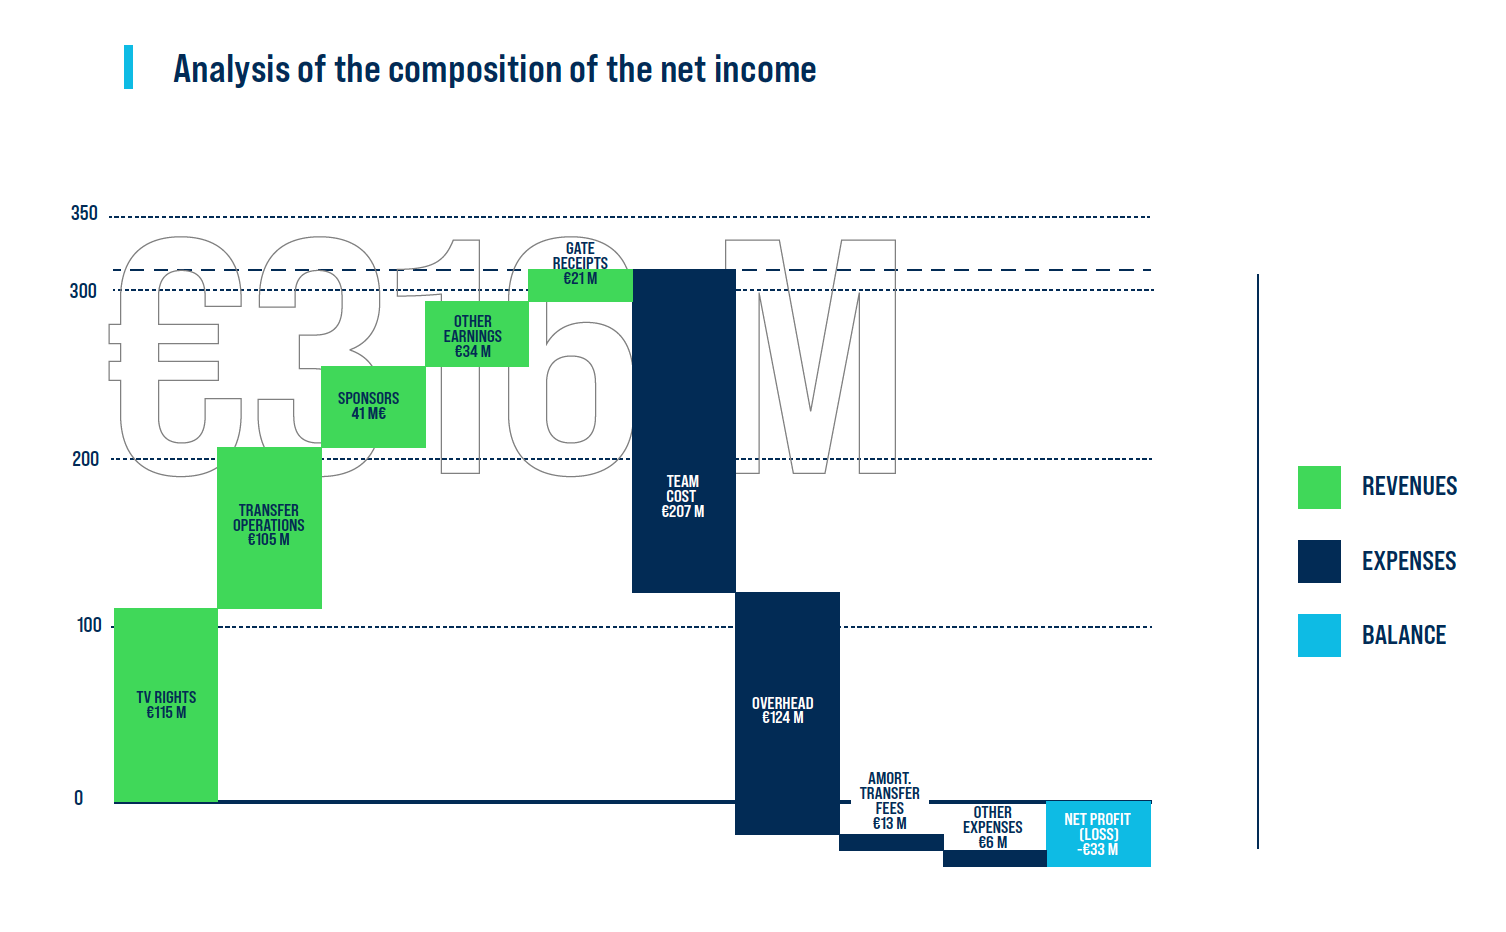
\includegraphics[width=.45\textwidth]{img/net_income_2019.png}}
    \caption{Comparazione Risultato Netto (Net Income)}
    \label{comp_income}  
\end{figure}

La perdita registrata nella stagione 18/19 \'e la seconda in termini di importanza a partire dalla stagione 2013/2014 e
il motivo principale che spiega questa discesa cos\'i decisa, \'e da attribuirsi ad un aumento delle entrate (\emph{Income}),
con un valore che passa da 304 mln€ nel 17/18 a 316 mln€ nel 18/19, che per\'o non riesce a controllare l'aumento pi\'u considerevole
delle spese (\emph{Expenses}), sopratutto nella parte dedicata alle spese dei club (stipendi di giocatori e commissioni degli agenti) 
e nella parte delle "Altre spese" (\emph{Other Expenses}) che aumentano rispettivamente di 5 e 9 mln€. Inoltre, osservando le due figure,
si pu\'o notare come nella prima stagione la parte di spese relativa ai club e la voce "Altre spese" andasse a portare a 0 il profitto,
mentre nella stagione successiva gi\'a solo queste due voci vanno a creare una perdita.\\
Un secondo indicatore che \'e possibile prendere in considerazione per questa prima analisi generale \'e il \emph{Payroll}. Con questo termine
si esprime lo stipendio anno di un club ed occupa vari punti all'interno dell'analisi pubblicata da DNCG. Nel nostro caso prendiamo 
in considerazione la figura \ref{stipendi_ligue1} che esprime il Payroll medio dei club a seconda della posizione che hanno raggiunto
in classifica. \'E possibile da subito notare cla differenza tra le squadre qualificate per la Uefa Europa League e quelle che hanno
raggiunto la Uefa Champions League abbiano una differenza di Payroll medio di 75,9 mln€ che, considerando la differenza di posizionamento 
in classifica (in generale massimo 3 posizioni), \'e un valore molto elevato. Sicuramente la colonna pi\'u a destra \'e composta in modo
considerevole dalla squadra Paris Saint Germain (oggetto di una trattazione successiva) che, grazie ai fondi Arabi, possono permettersi
stipendi di gran lunga maggiori della media delle altre squadre del campionato.
\begin{figure}
    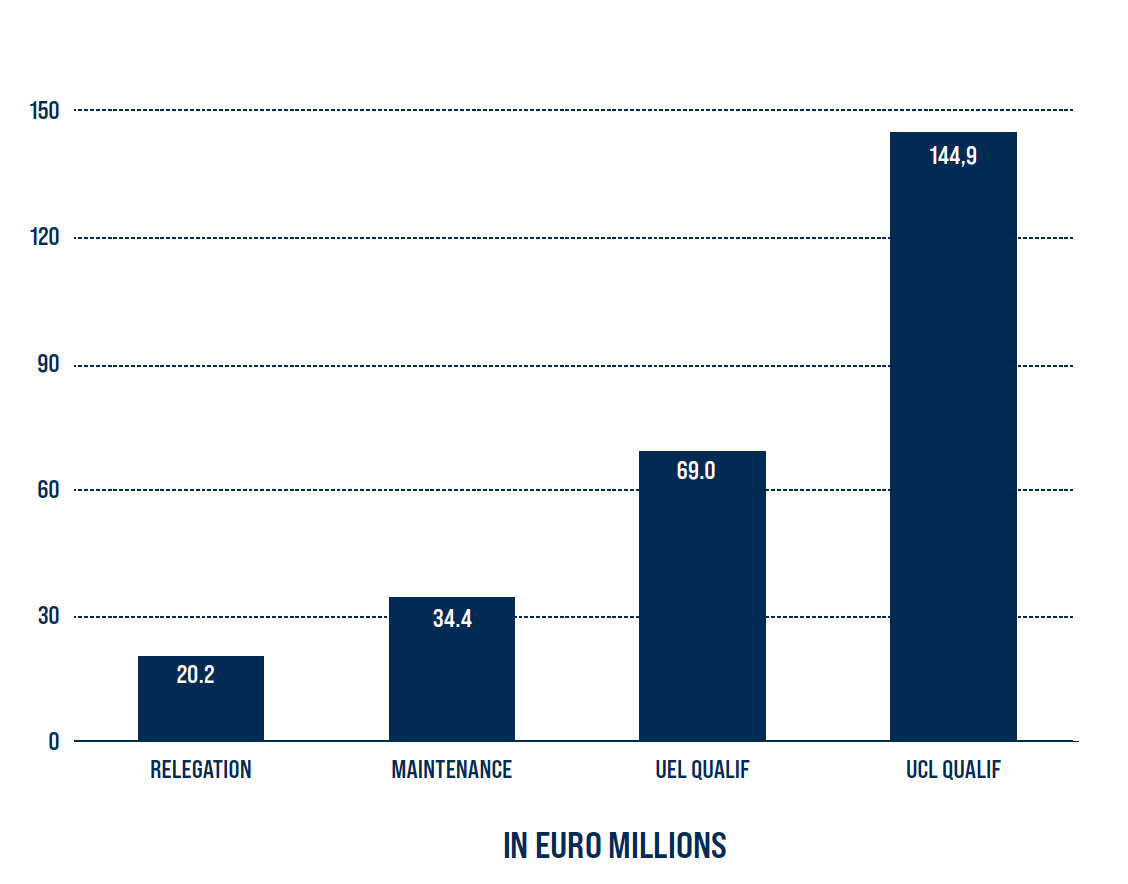
\includegraphics[scale=.5]{img/stipendi_ligue1.png}
    \caption{Stipendio medio dei club che occupano rispettivamente le diverse zone della classifica: zona retrocessione, 
    mat\'a classifica, qualificazione per Uefa Europa League e qualificazione per CHampions League}
    \label{stipendi_ligue1}
\end{figure}
%spiegazione finale su quello che è successo
\end{interlinea}





\end{document}

